% Simon Winther Albertsen: Table 1(e) loss-metric replication.
% Uses one experiment copy: ../meanflow-table1e-light/ (not independent of the full copy).
% Regenerate recorded assets: python analysis/analyse_loss_metrics.py from RAPPORT/.
% All ten endpoints must pass completion/config/source/evaluation checks.
% If a refreshed copy is incomplete, retain pending labels and do not use a complete
% two-seed table. The script prints pending run paths and withholds its aggregates.
% Preserve seed 42 and every seed-43 endpoint; never select the best epoch or seed.
% Recompile and inspect the one-page layout after any update. Simon's contributions
% to shared discussion/conclusion use the same verified two-seed endpoints.

\section{Experiment: adaptive loss metrics}
\label{sec:loss-metrics}

We reproduce MeanFlow's Table~1(e)~\cite{meanflow} to test whether adaptive loss weighting improves one-step FID and whether $p=1$ performs best among $p\in\{0,0.5,1,1.5,2\}$. We train ten models: two per $p$, with training seeds~42 and~43. Within each sweep, only \texttt{method.norm\_p} varies.

\textbf{Objective and controls.}
For training example $i$, let $q_i=\|u_\theta-\operatorname{sg}(u_{\mathrm{tgt}})\|_2^2$, summed over latent elements. The released code minimizes
\begin{equation}
  \mathcal{L}_p=\frac{1}{B}\sum_{i=1}^{B}
  \operatorname{sg}\!\left[(q_i+c)^{-p}\right]q_i,
  \qquad c=0.01,
  \label{eq:adaptive-loss}
\end{equation}
Here $\operatorname{sg}$ stops gradients through the Jacobian-vector-product target and adaptive weight. Setting $p=0$ gives squared L2 loss; $p>0$ downweights larger residuals. We use the released \texttt{norm\_eps}=0.01. Training-loss scales vary with $p$ and are not compared.

We use class-conditional MeanFlow/DiT-B/4 (131.2M parameters), trained from scratch for 80 epochs (400,320 updates) with global batch~256 on one NVIDIA B200 per run. AdamW uses a constant learning rate of $10^{-4}$, $(\beta_1,\beta_2)=(0.9,0.95)$ and zero weight decay; EMA decay is 0.9999. All runs use FP32, logit-normal time sampling $(-0.4,1.0)$, $r\ne t$ for 25\% of examples, $(t,t-r)$ conditioning, class dropout~0.1 and no classifier-free guidance.

\textbf{Implementation and evaluation.}
We use the authors' JAX code~\cite{meanflow-code}, commit \texttt{d70cb55}. We encode ImageNet-1K's 1,281,167 training images, center-cropped to $256\times256$, with the pretrained VAE \texttt{pcuenq/}\allowbreak\texttt{sd-vae-}\allowbreak\texttt{ft-mse-flax} at revision \texttt{7581b0a}. We sample $32\times32\times4$ latents from cached posterior means and standard deviations, with scaling~0.18215. We evaluate EMA FID on 50,000 decoded images every ten epochs with one network evaluation (1-NFE), fixed sampling seed~0, and the authors' JAX Inception/resize pipeline and reference statistics. We report epoch~80, averaging the two measured FIDs without pooling sample statistics.

\begin{table}[!ht]
  \centering
  \caption{Epoch-80 EMA FID-50K (1-NFE), mean $\pm$ sample SD ($n=2$ training seeds, ddof=1). $\Delta=\text{paper}-\text{our mean}$. Bold marks minimum FID per column.}
  \label{tab:loss-metrics}
  % Generated by analysis/analyse_loss_metrics.py; epoch 80 only.
% Delta = paper FID minus our two-seed mean; bold marks minimum FID.
\begingroup
\setlength{\tabcolsep}{4pt}
\begin{tabular}{@{}crrrrr@{}}
\hline
$p$ & Paper & Seed 42 & Seed 43 & Mean $\pm$ SD & $\Delta$ \\
\hline
0.0 & 79.75 & 80.23 & 81.47 & $80.85 \pm 0.88$ & $-1.10$ \\
0.5 & 63.98 & 64.60 & 65.22 & $64.91 \pm 0.44$ & $-0.93$ \\
1.0 & \textbf{61.06} & \textbf{61.36} & \textbf{61.44} & $\mathbf{61.40} \pm 0.06$ & $-0.34$ \\
1.5 & 66.57 & 67.32 & 66.62 & $66.97 \pm 0.49$ & $-0.40$ \\
2.0 & 69.19 & 97.61 & 97.95 & $97.78 \pm 0.24$ & $-28.59$ \\
\hline
\end{tabular}
\endgroup

\end{table}

\begin{figure}[!ht]
  \centering
  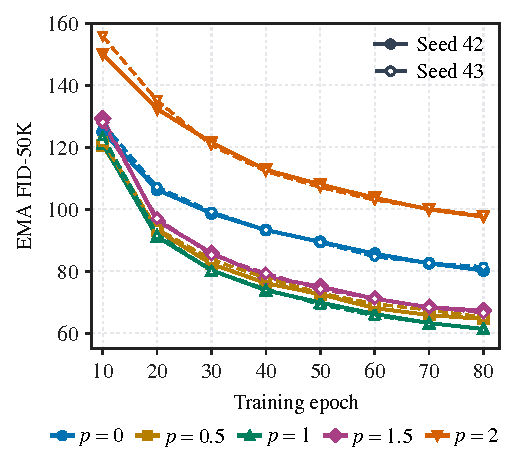
\includegraphics[width=\columnwidth]{figures/loss_metrics_fid_epochs.pdf}
  \caption{Recorded EMA FID-50K at ten-epoch checkpoints. Colour identifies $p$; solid/filled denotes seed~42, dashed/open seed~43. Paired curves largely overlap.}
  \label{fig:loss-metrics-curves}
\end{figure}

\begin{samepage}
The TPU release pins JAX/JAXlib~0.4.27; our GPU runs use~0.11.2, Python~3.12.3, Flax~0.12.10 and SciPy~1.18.1. Patches adapt JAX/SciPy APIs, single-process startup, local VAE loading and data-loader workers; a wrapper records results and timings. We freeze latent file order; epochs repeat that order without latent flips, as in the released loader. Historical training seeds, file order and stabilizer values are unspecified, preventing bitwise historical replication.\par
\end{samepage}

\textbf{Results.}
Setting $p=1$ is best in both seeds, with mean FID $61.40\pm0.06$ (Table~\ref{tab:loss-metrics}). For $p\leq1.5$, individual scores are 0.05 to 1.72 above the paper. For $p=2$, FIDs are 97.61 and 97.95 versus 69.19; their mean exceeds the paper by 28.59 and performs worse than our $p=0$ results. Both seeds' FIDs decrease at every checkpoint, with $p=2$ highest throughout (Figure~\ref{fig:loss-metrics-curves}). This is partial numerical replication; the persistent $p=2$ discrepancy has no identified cause.

Recorded run time totals 63.03 GPU-hours: 31.61 for seed~42 and 31.42 for seed~43. Runs take 6.281 to 6.325 hours; parallel sweeps take 6.33 and 6.29 elapsed hours, respectively. Timings include compilation, I/O, evaluation, checkpointing and recording; preprocessing and idle allocation time are excluded. Allocated/billed time is unavailable. Eight FID evaluations take 21.1 to 25.1 minutes per run; median logged throughput from step~500 is 18.97 to 19.07 updates/s.

After inspecting seed~42, we repeated the full sweep with only the training seed changed to~43 to check sensitivity to training randomness. All ten runs completed successfully. Two seeds provide limited descriptive evidence and cannot establish robustness, significance or outlier status.
